\documentclass[12pt]{article}
\usepackage[utf8]{inputenc}
\usepackage{graphicx}

\title{DD Lab 9 Assignment}
\author{Sai Kartik \\2020A3PS0435P}

\begin{document}
    \maketitle
    \section*{Circuit diagram in the no change state}
    \begin{figure}[ht]
        \centering
        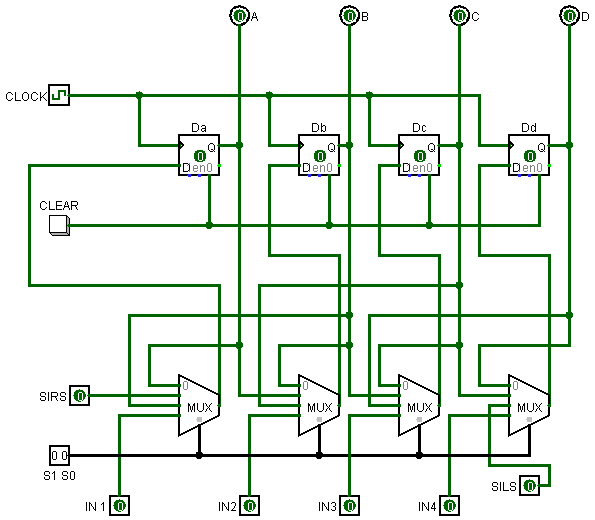
\includegraphics[scale=0.50]{nochange.png}
        \end{figure}
    \newpage
    \section{Circuit diagram in the load state}
    \begin{figure}[ht]
        \centering
        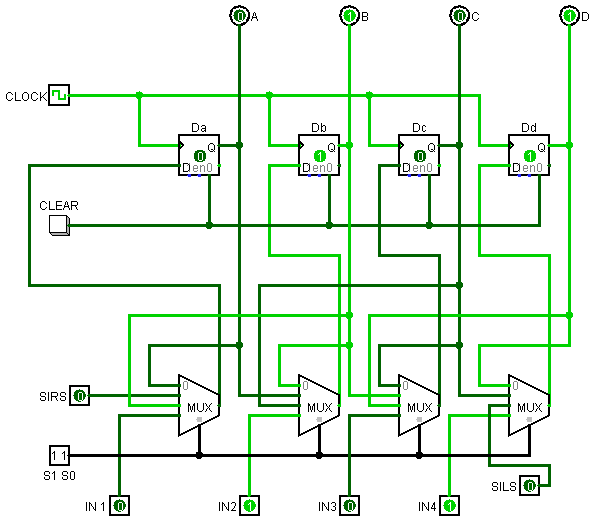
\includegraphics[scale=0.50]{load.png}
    \end{figure}
    \newpage
    \section{Left shifting the loaded register}
    \begin{figure}[ht]
        \centering
        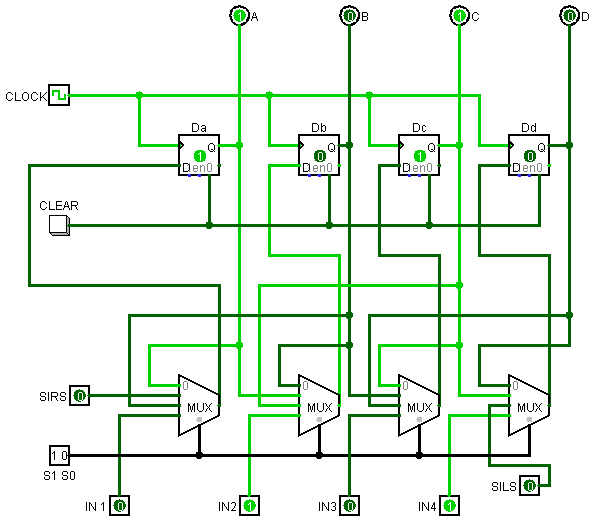
\includegraphics[scale=0.50]{leftshift.png}
        \caption{Left shifting once}
    \end{figure}
    \newpage
    \section{Right shifting the initial loaded register twice}
    \begin{figure}[ht]
        \centering
        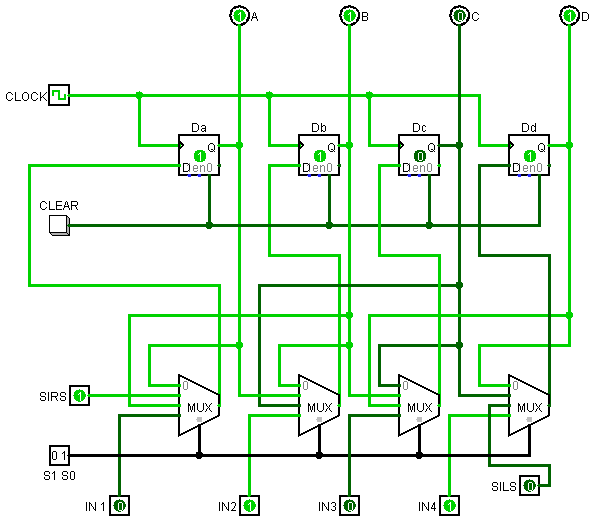
\includegraphics[scale=0.50]{rightshift.png}
        \caption{Right shifting twice}
    \end{figure}
\end{document}